\section{Neutrale Netzwerke von RNA-Strukturen (Peter Schuster)}

Diese Methode erlaubt Aussagen über die Evolvierbarkeit von Strukturen zu formulieren. Es gibt konservierte Strukturen, welche stabil gegen Mutation sind. Für neutrale Netze ist festgelegt, dass aus einem neutralen Netz alle weiteren neutralen Netze mit einer Mutation erreicht werden können.

\subsection{Shape-Abstraktion (R. Giegerich)}

Simplifizierung einer Sequenz um diese vergleichbar mit anderen Sequenzen zu machen. Erzeugung sogenannter suboptimaler Shapes:
\begin{itemize}
\item \ ((.(((...)))....((((.....))))..(.((..))).)) (Ausgangszustand)
\item \ [.[.].[.].[.[.]].]
\item \ [.[.].[.].[.].] 
\item \ [[][][]] (stärkstes sinnvolles Abstraktionslevel)
\end{itemize}

\textbf{SHREP} = SHape REPresentatives: Als Ergebnis wird die Wahrscheinlichkeit der besten Struktur der Shapes ermittelt.

\subsection{Faltungskinetik mit Energielandschaften}
\textbf{Kinetische Überlegungen im Falten von RNA:}
\begin{itemize}
\item Moleküle in biologischen Systemen liegen meistens nicht im thermodynamischen Gleichgewicht \\
$\rightarrow$ Entstehung von kinetischen Fallen == minimum free Energy (tiefe lokale Minima in der Energielandschaft)
\item kinetische Fallen können zum Beispiel durch RNAi (cotranskriptionales Falten) erzeugt werden
\item sogenannte RNA-Schalter wechseln von einem lokalen Minimum in ein anderes und falten somit absichtlich von einem in den anderen Zustand \\ $\rightarrow$ metastabile RNA-Faltungszustände (erzeugen zusätzlichen Regulationsfaktor)
\item freie Energie pro Struktur
\item Wahrscheinlichkeit für bestimmte freie Energie $\Delta$G abhängig von der Zeit
\end{itemize}

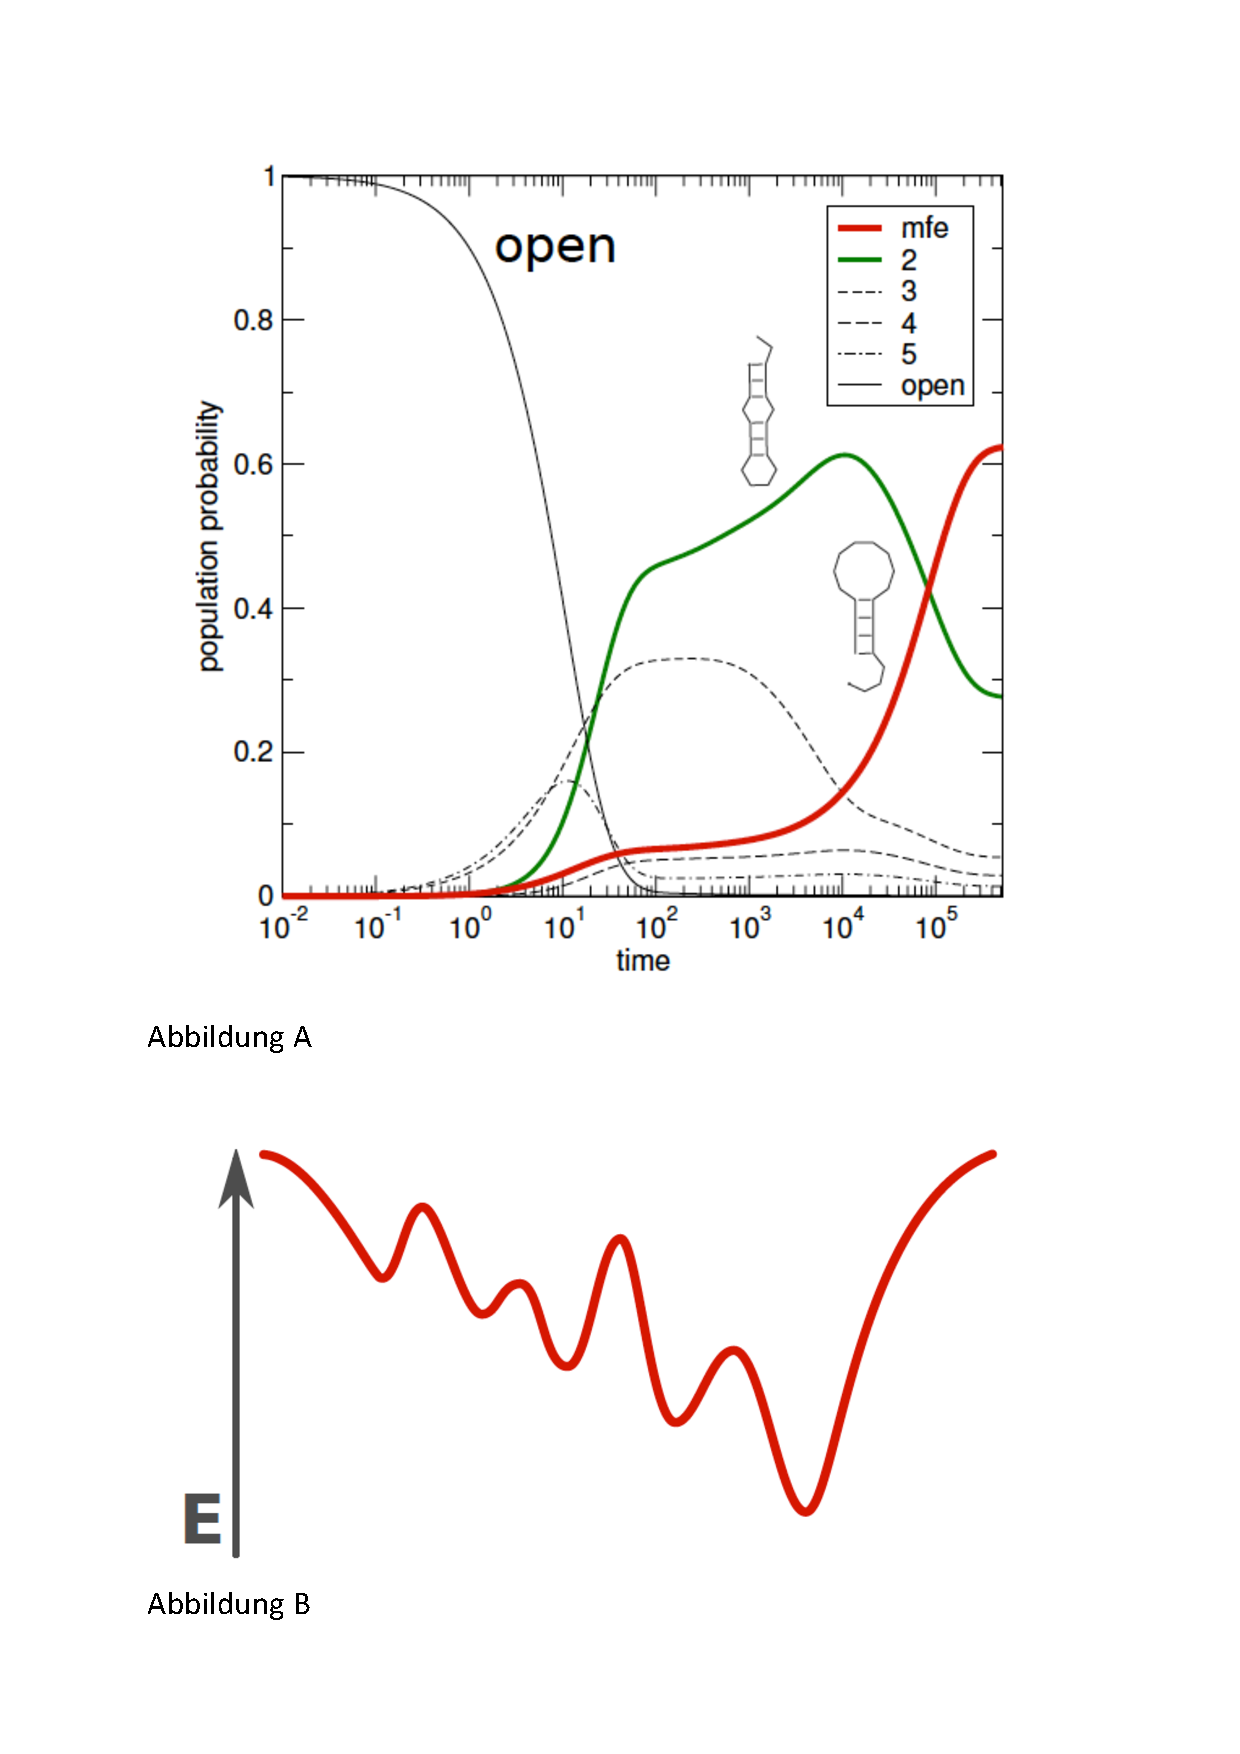
\includegraphics[scale=0.5]{lectures/160523/pix/Diagramme} \\
Abbildung A zeigt die Wahrscheinlichkeit eine Struktur einer RNA-Sequenz zu bestimmter Rechenzeit zu ermitteln. Hierbei zeigen die verschiedenen Kurven verschiedene Bereiche der Energielandschaft. Rot entspricht der minimalen freien Energie. \\
Abbildung B zeigt eine Energielandschaft, also die energetischen Niveaus einer RNA-Sequenz in Abbhängigkeit ihrer Strukturzustände. \\

\textbf{Erlaubte Schritte sind} (Move-Set): 
\begin{itemize}
\item öffnen von Basenpaaren
\item schließen von Basenpaaren
\item Verschiebung von Basenpaarteilen
\end{itemize}

\subsubsection{Metropolis-Monte-Carlo}
Die Anzahl zu betrachtender Zustände ist zumeist viel zu groß, weswegen mit stochastischen Methoden, wie Monte-Carlo und oder Markov-Prozessen gearbeitet werden muss. \\
Ein Schritt in Richtung niedriger Energie ist leichter als in Richtung höherer Energie. \\ 
Nachteil: Methode funktioniert nur für kleinere Probleme zufriedenstellend $\rightarrow$ grobkörniger Ansatz nötig: Erzeugen einer Übergangsmatrix k (exponentielles Wachstum) oder helixbasierte Move-Sets \\
Im ersten Schritt wird ein Zustandswechsel i $\rightarrow$ j vorgeschlagen. Überprüfe, ob \textbf{Zustand} besser ist $\rightarrow$ Metropolis-Regel: \\
\begin{equation}
p_{Akzeptanz}(i,j) =
\begin{cases}
e^{-\dfrac{G_j - G_i}{RT}} \ if \ G_j > G_i \\ 1 \ \ else \\
\end{cases}
\end{equation}
alternativ Kawasaki-Regel: \\
\begin{equation}
K_{ij} = e^{-\dfrac{G_j - G_i}{2RT}}
\end{equation}

Voraussetzung: i und j sind benachbart (?wie auch immer das bei Zuständen gemeint ist?)

\subsubsection{Barrier-Trees}
\begin{itemize}
\item[1] Berechnung aller suboptimalen Strukturen des Energiebandes ($\rightarrow$ Wuchty-Algorithmus) 
\item[2] Bauen eines Baums aus allen suboptimalen Strukturen
\item[3] Faltungspfad zwischen Strukturzuständen i und j $\rightarrow$ Sequenz von erlaubten Schritten, die aus Anfangsstruktur i die Endstruktur j erzeugt
\item[4] Wahl des optimalen Faltungspfads: Faltungspfad mit minimalen Maximum der Energie der Strukturen, die besucht werden
\end{itemize}
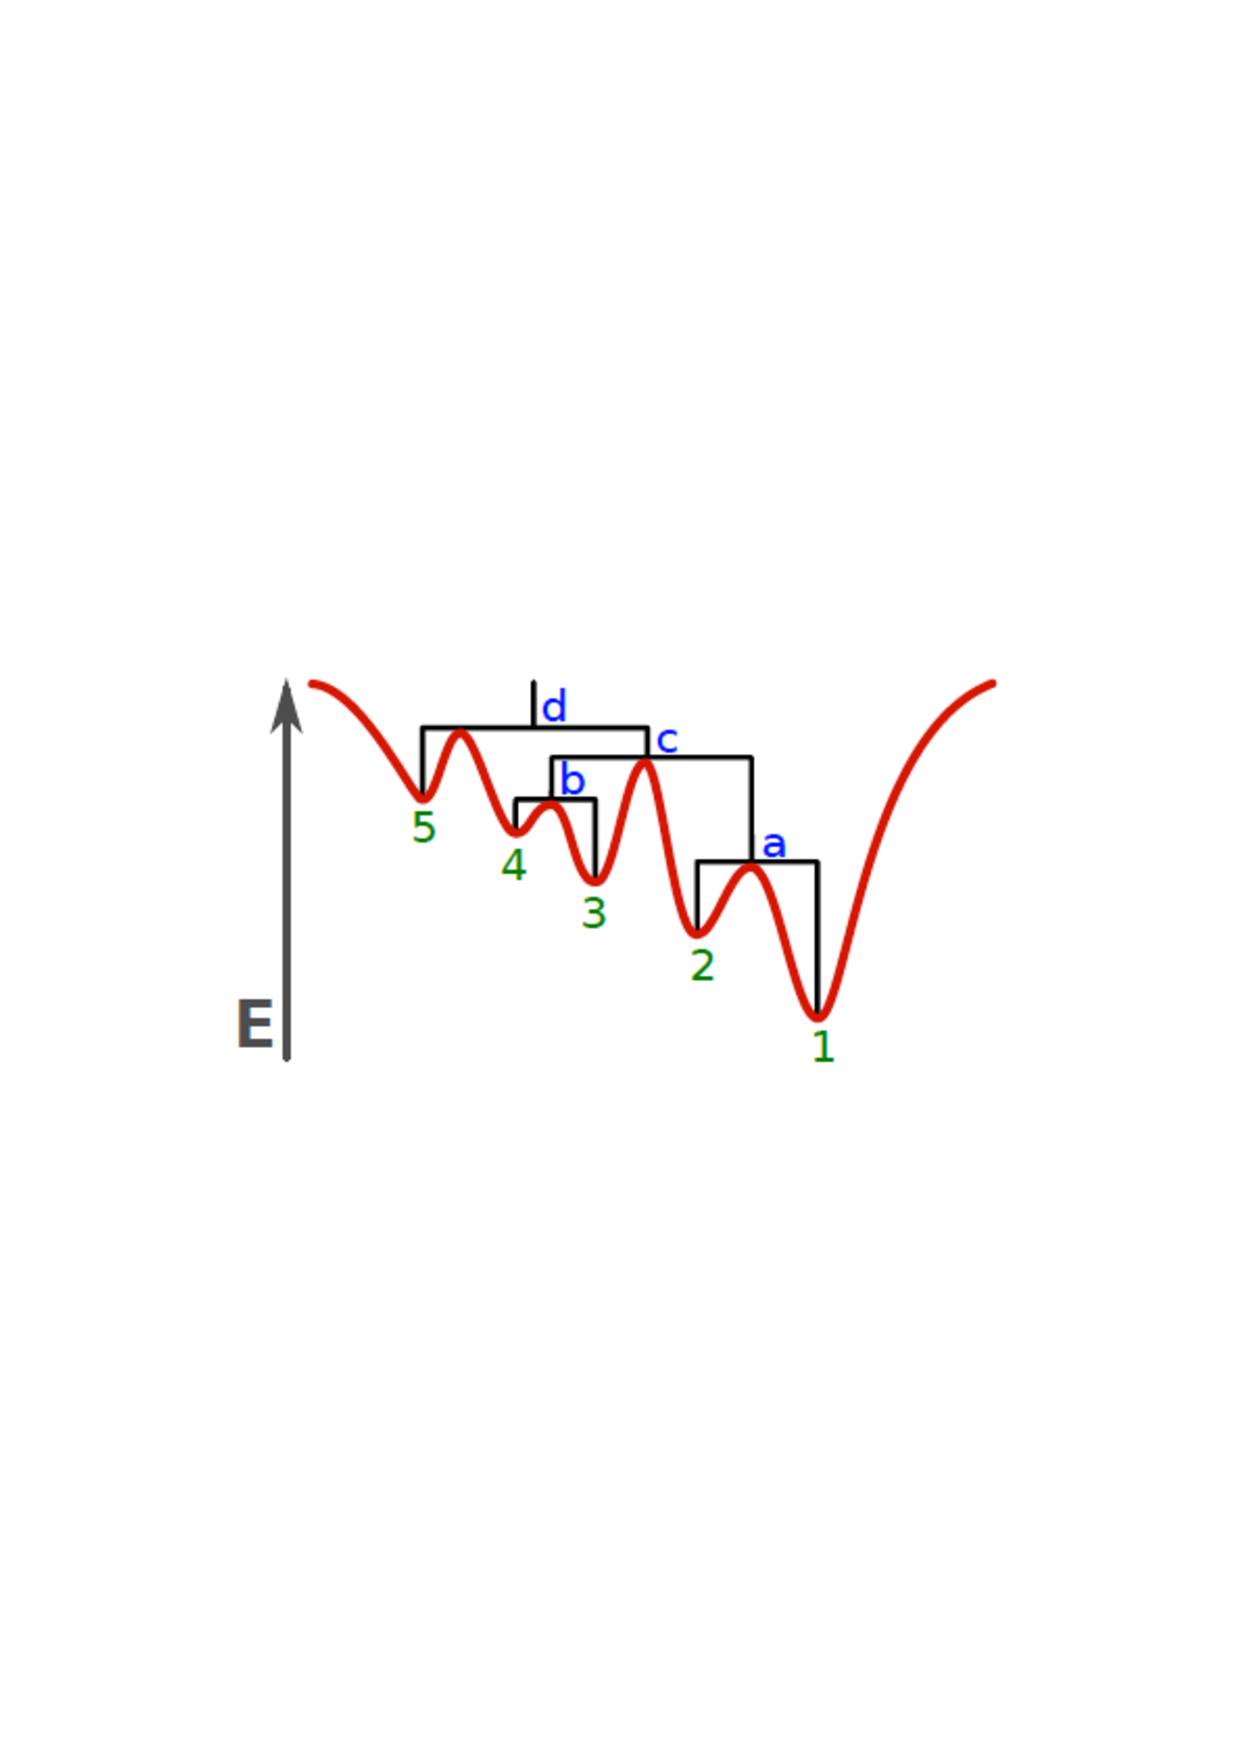
\includegraphics[scale=0.7]{lectures/160523/pix/Barrier-Tree.pdf} \\
Die Abbildung zeigt einen Barriertree, der aus den Minima und den Sattelpunkten der Energielandschaft erzeugt wurde. 

\subsubsection{Baumbau mit Flooding-Algorithmus}
Erzeugung einer Strukturliste, die nach Energiewerten sortiert ist. Diese wird dann als Hash eingespeichert.\\
besuchte Struktur $\rightarrow$ Niveaunummer
\begin{itemize}
\item Beginn bei Struktur 0 mit Niveaunummer 0
\item Besuchen aller Nachbarn $\rightarrow$ Überprüfe im Hash
\begin{itemize}
\item[a] gibt es keinen Nachbarn im Hash $\rightarrow$ neues Minimum im Hash 
\item[b] haben alle die selbe Niveaunummer $\rightarrow$ alle gehören einem Hash an
\item[c] Nachbarn in zwei Niveaustufen $\rightarrow$ Sattelpunkt an der Stelle wo beide Niveaus zusammenkommen
\end{itemize}
\item Berechnung der Wahrscheinlichkeit nach Arrhenius:
\begin{equation}
p(x,y) = A*e^{-\dfrac{E_{Sx}-E_{Sy}}{RT}}
\end{equation}
\end{itemize}

\subsubsection{Direkte Pfade}
Die Nutzung direkter Pfade stellt eine Alternative zum Flooding-Algoithmus dar.\\
Gegeben sind zwei Sets von Basenpaaren (A,B)\\
a $\rightarrow$ b: erlaube nur Verschiebungen, die entweder Basenpaare A außer B wegnehmen oder ein BP aus B außer A hinzufügen. \\
Heuristiken zur Bestimmung von guten direkten Pfaden:
\begin{itemize}
\item[1] Morgan-Higgs-Heuristik: Wahl des besten Schritts
\item[2] Find-Path-Heuristik: Generiere alle möglichen Schritte und wähle davon die fünf besten aus
\end{itemize}

\subsubsection{Cotranskriptional Folding}
Programm: KinWalker \\

Barmap-Ansatz:
\begin{itemize}
\item[1] Zufälliges Wählen eines Barrier-Tree
\item[2] Simulieren des Barriertrees auf einen neuen Tree und damit die Energielandschaft abändern
\item[3] Mappe die Niveaus von Barrier-Tree I zu denen von Barrier-Tree II
\item[4] Erneut zu Punkt 2 und mit Barrier-Tree II weitersimulieren 
\end{itemize}